\documentclass[12pt, a4paper]{article}
\usepackage{graphicx}
\graphicspath{{./images/}}

\title{Sound rendering and envelope development for music generator in Clean}
\author{Beka Grdzelishvili}
\date{January 2020}

\begin{document}

\maketitle

\section{Introduction}
In music, an envelope describes the varying level of a sound wave over time. It is the envelope of a wave which establishes the sound’s uniqueness, it has a significant influence on how we interpret music. Classic envelopes consist of 4 main parts: Attack, Decay, Sustain and Release, where sustain refers to level, while others represent time interval. Attack is the period of time which sound needs to reach its peak from zero, after the key is pressed. After the attack starts decaying period, when sound level decreases to sustain level, and stays unchanged, during sustain phase, until the key is released. Final phase of the envelope is the release, which begins when sustain phase ends and continuous until sound fades to silence. Almost every musical instrument has own individual envelope, for example a quick attack with little decay makes sound similar to organ, while a longer decay is characteristic of a guitar. In this project, envelope generator, which is common feature of synthesizers and electronic musical instruments to control the different stages of a sound, was developed for music generator wrote in Clean using pure functional programming.

\section{Implementation of Envelopes with List}

Purpose of the envelope generator function is to calculate values for envelope according to the given parameters. Those functions take note data and corresponding values for each step of the envelope as arguments and generate list of real numbers, which take values from -1.0 to 1.0. In this implementations values are stored in List data structures. To make function more efficient List comprehensions and lazy evaluation, Clean’s two main advantages, are actively used during calculations. For each type of envelope corresponding Record structure was developed for easily manipulating envelope data. Each record contains information about duration, level and/or rate of each step according to which final list is created. 

\subsection{ADSR Envelope}

\textit{getADSR} function is used to generate ADSR Envelope. It has only basic 4 steps: Attack, Decay, Sustain and Release. Function gets beat, time signature, tempo and ADSR record as parameters. At first beat, time signature and tempo are used to calculate the duration of the note, time interval between pressing and releasing the key. \textit{noteToSamples}, one of the utility functions, is used to convert these parameters to the number of samples in this time interval. After that, number of samples for each step of envelope is calculated. As the release is independent from the note duration it is enough to directly convert given release duration to samples, but other 3 steps need different approach. Instead of directly using given duration of each step independently, number of samples are calculated based on time offset from the starting time and subtracting sum of samples of the previous steps (As sustain does not have fixed time interval, total note duration can be used as offset). This is important to avoid losing samples during flooring of real numbers and to make sure that number of total samples is equal to sum of each step’s samples. After calculating list of samples of each step are calculating independently using list comprehension. For the linear attack and decay value of sample is instantly calculated with index, number of samples and final value. Concatenating these lists gives whole envelope except release tail, but as key might be released any time during first 3 step, even during attack or decay, we might need to shorten it. Clean built in function take is used to take exact amount of samples needed. Finally release tail list is generated in the same way as attack and decay and is concatenated to others to get complete envelope. 

\begin{figure}[ht!]
\centering
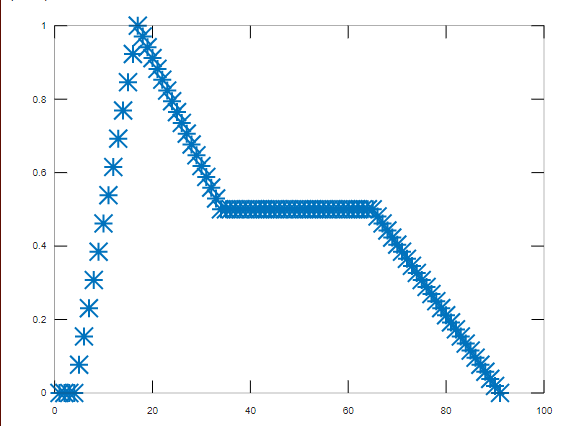
\includegraphics[scale=0.3]{env1}
\caption{ADSR Envelope}
\end{figure}

\subsection{DAHDSR Envelope}

\textit{getDAHDSR} function generates another type of envelope, which has two more steps then ADSR envelope: delay and hold. Delay is the time interval before attack, when sound stays silent, while hold phase comes after attack and indicates duration while sound maintains its peak. Functions implementation is similar to \textit{getADSR} function. Each step is generated using list comprehensions and concatenated. Whole envelope is generated and only after that its prefix is taken to make sure that key can be released at any time.

\subsection{Casio, 8 step Envelope}

Casio is a more modern type of envelope, which allows more flexibility and vast variety of envelopes. It is different from above mentioned types, for each step, instead of providing duration and level, it has 8 steps, described by rate and level values, where level is the desired percentage to be reached at the end of the current phase, while rate denotes the percentage with which samples change per second. Rate and level pair make possible for same phase to be ascending or descending depending on the needs of users. Implementation of Casio envelope differs for other two envelopes, as the structure is different. \textit{CasioCZ} record provides data, necessary for creating Casio envelope, it has rate and level values for each 8 step, first 5 step represent front part of the envelope, while last 3 steps are used to generate release tail after sustain. \textit{generateLine} function is used to generate point values for line between two level using current rate. This function returns not  list of points, but tuple of list and real value. Second return value plays important role in interpolation. Last value of line, may not have integer index, hence it can not be included in the list. Due to the above mentioned reason, instead of directly using previous endpoint as the beginning for the current line we need to recalculate it based on the second value of generateLine function using the formula: \(casio.level1-rt2*(snd  line1)\). At the end, similarly to other envelopes, we need to take exact amount of samples according to note duration.

\subsection{Generalized Envelope}

Last type of envelope data structure is Generalized Envelope, which is similar to Casio envelope, but provides even more flexibility during sound synthesizing. It is similar to Casio envelope with it’s structure, both of them use rate and level values to describe each step, but generalized envelopes do not have fixed amount of steps like other previous structures. \textit{GenEnv} record uses list to store data, where each element is \textit{EnvLevel} record type, containing rate and level values. Also, as generalized envelopes do not have fixed number of steps before release tail, \textit{GenEnv} record contains value for index indicating sustain level. Generating data for each step is done similarly to Casio envelope, but rate and starting value can not be recalculated manually, so we need to preprocess data before using it. \textit{parseData} function is used to recursively traverse initial list and generate new one, which can be directly used to generate lines for each step using same way as in Casio envelope. 

\section{Efficiency improvements}

Unlike other steps release does not have fixed starting value and it needs to be calculated based on the time of releasing key. First implementation of envelope generator function used last, built in functions for list, to calculate base value of release. As lists are implemented as linked lists and do not have direct access to the element last function uses recursive approach which resulted in \(O(N)\) time complexity and excessive use of memory. To avoid overfilling heap memory release base value was calculated directly using constant time and memory. At first it is determined on which step generation was terminated and then value can be calculated directly according to it. 

\section{Implementation of Envelopes with Arrays}

As mentioned before, lists are similar to linked lists, therefore they do not provide direct access to the elements. During usage of envelopes it might be essential to have direct access to avoid linear time complexity and provide better memory management, therefore envelope generator functions were also implemented with arrays instead of lists. These implementations provide direct access to data and support array implementations of waves, which can be handful, for example, during summing up different waves, while this can not be done with lists, at first they need to be converted into arrays, then processed and reconverted to the lists again.

\section{Rendering waves and applying envelope}

Rendering process consists of several steps. First step is to calculate whole length of the sound, as each wave can start at different moment of time and can have distinct lengths. This value will be used later, to generate silent track, which will act as the base during summing up all wave samples.  Next step is to process data stored in each chunk to generate sound waves and sum up all of them. Each chunk stores wave type, time signature, tempo, envelope and other data, extracted from MIDI files, which are needed to generate wave and apply envelope to it. Values for each wave can be calculated using already developed functions for envelopes and sound synthesizing. After generating all waves we need to sum up them in the single list. If we use arrays we can use each wave’s starting time as an index offset, but same approach is not useful with list implementation. To easily sum up lists they need to be same size, therefore appropriate amount of silence samples should be appended on the both sides of the list. Last step is normalization: converting values to \([-1.0, 1.0]\) range. After summing up lists some samples might go out of those bounds, that’s why final list needs to be normalized at the end of the process. After normalization sound rendering is finished and it can be used for later processing.

\begin{figure}[ht!]

\center
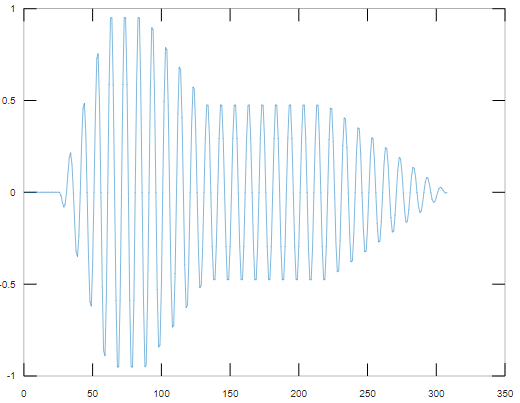
\includegraphics[scale=0.3]{sine1}
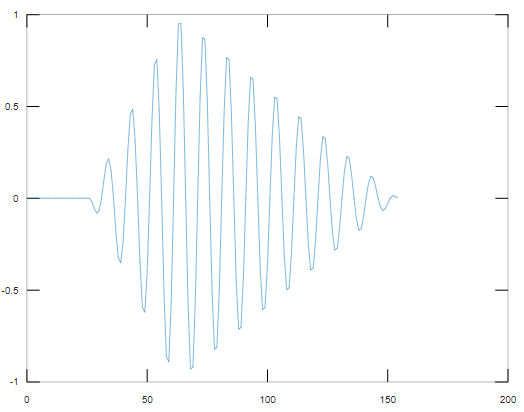
\includegraphics[scale=0.3]{sine2}
\caption{Sine wave modifed by different envelopes}

\end{figure}

\section{The End}

4 data structures were created to support different types of envelopes: ADSR, DAHDSR, Casio and Generalized envelopes. Several implementations and types of envelopes provide flexible environment during music generator development and sound synthesizing. Giving possibility to implement more efficient approaches during rendering process and creating envelopes to generate more complex and better sounds.

\end{document}